\chapter{Problem Definition and Existing Solution}

\section{Problem Definition}
Web-automation execute given natural-language task (for example, "book a one-way flight from Ahmedabad to Delhi on 12th May") in browser without human interaction following privacy and security. Agent process each task in steps to mitigate the intended outcome and At each step the agent has to output values of element, action, value. where the element is a DOM node on the page, the action is what to do at particular steps (click, type, select, and a few others), and the value is a string or null depending on the action. The steps are observable in two ways, the rendered screenshot and the HTML/DOM tree of that page. Current automation systems made around this to perform geven natural task in autonomous manner.

Three practical constraints turn this into a hard problem. First, modern pages contain 10,000 to 100,000 of DOM tokens \cite{zhang2025prune4web}, which is larger than the input context window of most LLMs as well expensive to send these many tokens on every step. Second, the agent has to execute a sub-task at low latency, otherwise the interaction does not feel live. Third, DOM elements in real websites carry user-sensitive values, such as email addresses, phone numbers, credit card fields, and identification numbers, so privacy and security concerns should be fulfilled with user awareness. A web-automation system therefore has to, reach high element-level accuracy while keeping low token cost, latency, and privacy risk.

Many paper has contributed in this topic, including SeeAct \cite{SeeAct}, which proposed a GPT-4V driven multimodal agent and introduced the Multimodal-Mind2Web dataset. SeeAct provided seperate planner and grounder concept at defined manner and thus used by further studies, but it relies on GPT-4V at every step, which makes reproducing the full SeeAct pipeline infeasible from a cost point of view.  

\section{Existing Solution: Prune4Web}

Prune4Web \cite{zhang2025prune4web}, is a three-stage pipeline for LLM-based web agents. Prune4Web solve the problem defined in SeeAct of low graounding rate and high interence cost using DOM prunining with better effective solution using weighted scoring implemntation. It is the closest published system to the design we want and it explicitly targets the cost/context problem of sending the DOM to the LLM. Figure \ref{Prune4Web:Architecture} shows the high-level flow.

\begin{figure}[!h]
    \centering
    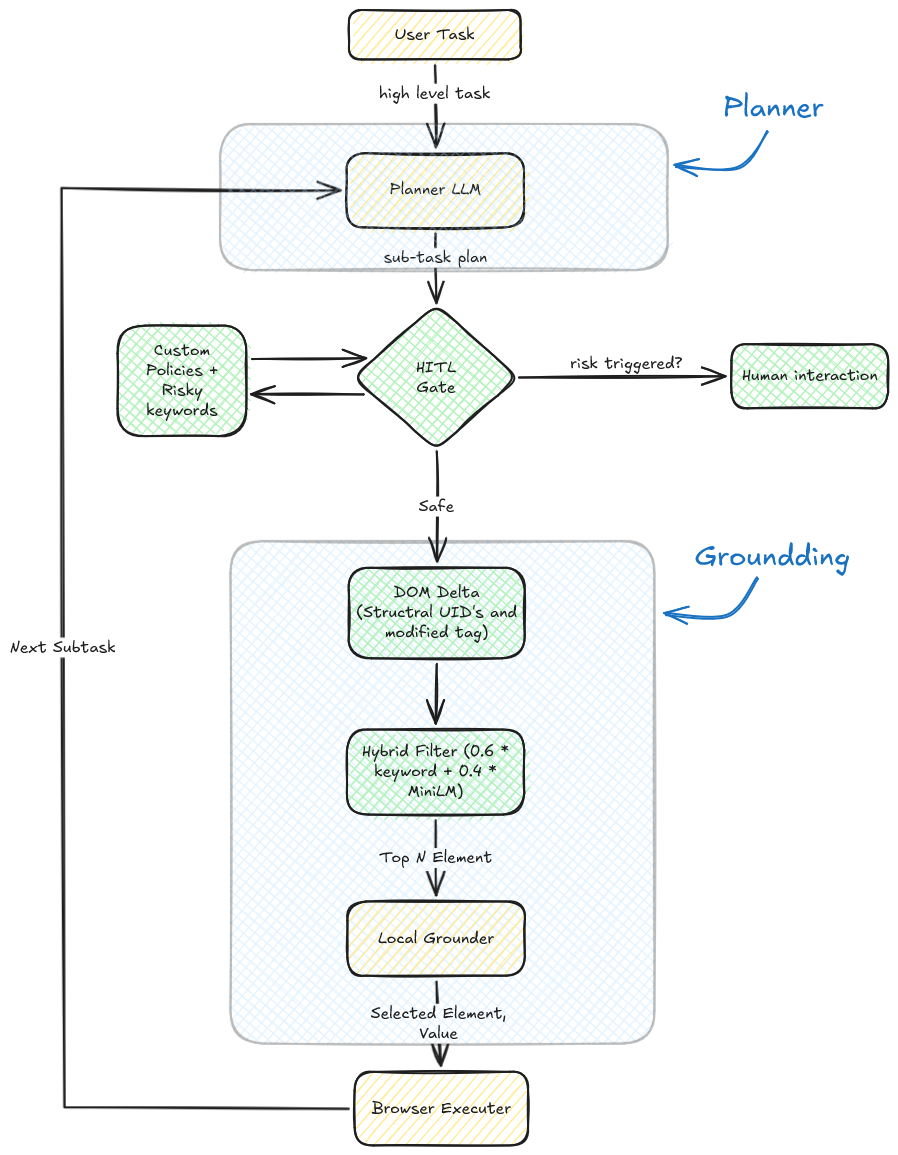
\includegraphics[width=0.6\linewidth]{Architecture.png}
    \caption{Prune4Web pipeline: Planner (LLM) $\to$ Programmatic Element Filter (LLM emits weights, Python scores) $\to$ Action Grounder (On filtered top-$N$ elements)\cite{zhang2025prune4web}.}
    \label{Prune4Web:Architecture}
\end{figure}

    \subsection{Stage 1: Planner}
    Prune4web Planner also works like a typical planner. A multimodal LLM receives the high-level task as input, the page screenshot, and the previous-step history, and infers a single JSON object with one \texttt{sub\_task} field, \texttt{action\_type}, \texttt{value}, and a short \texttt{reasoning} string. At each step, planner convert high level task like "buy a laptop under 50{,}000" into one executable sub-task, for example "click the search box" \cite{zhang2025prune4web}. The planner never looks at the raw DOM.

    \subsection{Stage 2: Programmatic Element Filter}
    This is the core contribution of the paper. The LLM is asked to generate a small set of keyword/weight scoring values based only on the sub-task, without seeing any DOM content. At this step, a sub-task by the planner given as input to the model, which is very small in terms of token size. A static Python scorer algorithm then uses that value and DOM element (tag, visible text, id, name, aria-label, placeholder, title, role, class) and returns the top-$N$ candidates \cite{zhang2025prune4web}. Because the LLM never reads raw DOM at this stage, the filter call stays $O(\text{sub-task length})$ in terms of tokens instead of $O(\text{page size})$, and the token usage reduces at 25x to 50x \cite{zhang2025prune4web}.

    \subsection{Stage 3: Action Grounder}
    A Typical Action Grounder receives the sub-task along with the filtered top-$N$ element summaries and returns the exact target (\texttt{element\_uid}, \texttt{action}, \texttt{value}). On Mind2Web, Prune4Web reports 88.28\% Element Accuracy with manually fine-tuned Qwen2.5VL-3B-Instruct, and shows that a lighter and local Qwen2.5-0.5B-Instruct variant also operates in the same Filter-Grounder pipeline \cite{zhang2025prune4web}.
    

\noindent Overall, Prune4Web also thinks of SeeAct architecture with planner and grounder with a new experiment of a defined novel DOM filter approach rather then using the DeBERTa model like SeeAct. Also it uses Mind2Web, which is the most standard available current benchmark across topics.


\section{Gaps We Inherit From Prune4Web}

Prune4Web over Mind2Web comes with three gaps that directly motivate the proposed contributions in Chapter 4.

\textbf{Grounder focused on a 3B vision-language model.}
Prune4Web's SOT 88.28\% Element Accuracy comes from a Qwen2.5VL-3B-Instruct grounder that the authors fine-tune themselves on the Multimodel dataset. A Qwen2.5-0.5B-Instruct variant is also used as a base model, but primary results are posted for the 3B model\cite{zhang2025prune4web}. Using a 3B VL grounder means the grounder always requires a 6GB local GPU where the model can load and infer, and the 0.5B text-only variant reported in the paper is not accompanied by LoRA hyperparameters. This create a gap whether a purely text-mode grounder below 1B parameters, trained with a documented methodology, can match the 3B VLM at element accuracy. Our QLoRA-tuned Qwen2.5-0.5B and Qwen3-0.6B grounders (Chapter 4 and 5) answer exactly that question.

\textbf{DOM processing is single-step and stateless.}
At each sub-task step of Prune4Web re-runs the filter on the full current DOM, even if the page has just changed a single node of the DOM or a few nodes of the DOM. A basic assumption we took that while interacting with the page, most of the time, the next step of the current step required only updated DOM nodes (for the clicked button on the dropdown, a new element will open the dropdown, and most likely we would need to interact there on the next step). Prune4Web, Mind2Web, AutoWebGLM, and D2Snap all share this limitation \cite{zhang2025prune4web} \cite{deng2023mind2webgeneralistagentweb} \cite{lai2024autowebglm} \cite{schiepanski2025d2snap}, and it is the gap that our DOM Delta Processing is designed to close.

\textbf{No privacy awareness for each sub-task level.}
Most Web-automation tools, including Prune4Web, do not look for sensitive pages like CAPTCHA, Payment-Gateway, login, or explicit privacy policies. Thus, they treat the sensitive pages the same as normal pages for automation. Both safety and privacy concerns are discussed as open problems in recent surveys \cite{tang2025surveymllmbasedguiagents} \cite{ning2025surveywebagentsnextgenerationai}, which we tried to solve using Privacy Hub + HITL layer in Chapter 4.

\bigskip
\noindent These gaps (local grounder, stateless DOM changes, privacy-aware execution) are the motivation for the proposed methodology described in Chapter 4 and evaluated in Chapter 5.

